\begin{figure} [h!]
\begin{center}

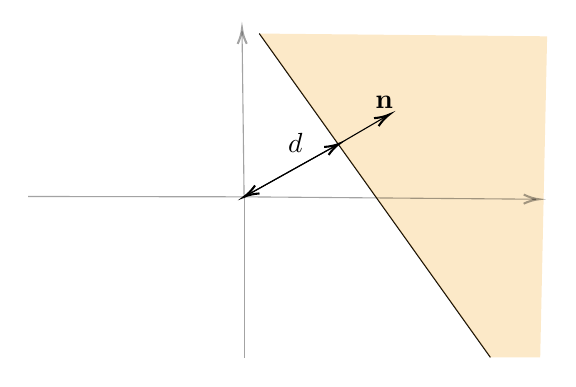
\begin{tikzpicture}[x=0.50pt,y=0.50pt,yscale=-1,xscale=1]
%uncomment if require: \path (0,300); %set diagram left start at 0, and has height of 300

%Straight Lines [id:da2789966724055237] 
\draw    (335,25.5) -- (502,259.5) ;
%Shape: Polygon [id:ds38542560237622214] 
\draw  [draw opacity=0][fill={rgb, 255:red, 245; green, 166; blue, 35 }  ,fill opacity=0.25 ] (543,27.5) -- (538,259.5) -- (502,259.5) -- (335,25.5) -- cycle ;
%Straight Lines [id:da1318799276011975] 
\draw    (324,143.5) -- (391.25,105.97) ;
\draw [shift={(393,105)}, rotate = 510.84] [color={rgb, 255:red, 0; green, 0; blue, 0 }  ][line width=0.75]    (10.93,-3.29) .. controls (6.95,-1.4) and (3.31,-0.3) .. (0,0) .. controls (3.31,0.3) and (6.95,1.4) .. (10.93,3.29)   ;
%Straight Lines [id:da16726546442154655] 
\draw    (393,105) -- (427.27,85.01) ;
\draw [shift={(429,84)}, rotate = 509.74] [color={rgb, 255:red, 0; green, 0; blue, 0 }  ][line width=0.75]    (10.93,-3.29) .. controls (6.95,-1.4) and (3.31,-0.3) .. (0,0) .. controls (3.31,0.3) and (6.95,1.4) .. (10.93,3.29)   ;
%Straight Lines [id:da3700435560461126] 
\draw [color={rgb, 255:red, 0; green, 0; blue, 0 }  ,draw opacity=0.36 ]   (324,143.5) -- (322.52,24) ;
\draw [shift={(322.5,22)}, rotate = 449.29] [color={rgb, 255:red, 0; green, 0; blue, 0 }  ,draw opacity=0.36 ][line width=0.75]    (10.93,-3.29) .. controls (6.95,-1.4) and (3.31,-0.3) .. (0,0) .. controls (3.31,0.3) and (6.95,1.4) .. (10.93,3.29)   ;
%Straight Lines [id:da802723255513649] 
\draw [color={rgb, 255:red, 0; green, 0; blue, 0 }  ,draw opacity=0.36 ]   (324,143.5) -- (324,260.25) ;
%Straight Lines [id:da6699382328755694] 
\draw [color={rgb, 255:red, 0; green, 0; blue, 0 }  ,draw opacity=0.36 ]   (168,143.25) -- (324,143.5) ;
%Straight Lines [id:da17215887220844728] 
\draw [color={rgb, 255:red, 0; green, 0; blue, 0 }  ,draw opacity=0.36 ]   (324,143.5) -- (535,145.23) ;
\draw [shift={(537,145.25)}, rotate = 180.47] [color={rgb, 255:red, 0; green, 0; blue, 0 }  ,draw opacity=0.36 ][line width=0.75]    (10.93,-3.29) .. controls (6.95,-1.4) and (3.31,-0.3) .. (0,0) .. controls (3.31,0.3) and (6.95,1.4) .. (10.93,3.29)   ;
%Straight Lines [id:da7790488401292512] 
\draw    (393,105) -- (325.75,142.53) ;
\draw [shift={(324,143.5)}, rotate = 330.84000000000003] [color={rgb, 255:red, 0; green, 0; blue, 0 }  ][line width=0.75]    (10.93,-3.29) .. controls (6.95,-1.4) and (3.31,-0.3) .. (0,0) .. controls (3.31,0.3) and (6.95,1.4) .. (10.93,3.29)   ;

% Text Node
\draw (417,69) node [anchor=north west][inner sep=0.75pt]    {$\mathbf{n}$};
% Text Node
\draw (354,96) node [anchor=north west][inner sep=0.75pt]    {$d$};

\end{tikzpicture}

\end{center} 
% \caption{Visualization of trajectory generation done in the developed software}
\end{figure}